\documentclass[12pt]{article}
\usepackage[left=2cm, right=2cm, top=2cm, bottom=2cm]{geometry}
\usepackage{graphicx}
\usepackage{float}
\usepackage{adjustbox}
\usepackage{amsmath}
\usepackage{amssymb}
\usepackage{commath}
\usepackage{wasysym}
\usepackage{pdfpages}

\title{CTA200 Project}
\author{Sinthushan Sivakumar}
\date{May $14^{th}$, 2021}

\begin{document}

\maketitle

\section{Introduction}
In this project the evolution of the Earth-Moon system was integrated back into the past, from present day configuration, using python 3 in a jupyter notebook. 

Ocean tides are caused by the gravitational attraction of the Moon, and to a lesser extent, the Sun. Lunar tides are known to increase both the length of day and the length of the Lunar month; the Lunar torque $-T_{\leftmoon}$ produced by the Moon’s gravity acting on the tidal bulge in the oceans and solid body of Earth reduces the spin angular momentum $S_{\oplus}$ of the rotating Earth, and adds the same amount to the orbital angular momentum $L_{\leftmoon}$ of the Moon, with no change in the sum $L_{EM} = S_{\oplus} + L_{\leftmoon}$. The solar torque $T_{\odot}$ associated with the solar tide increases both the length of day and the length of the year; it also reduces, very slightly, $L_{EM}$, increasing the orbital angular momentum $L_{\oplus}$ of Earth by the same amount:
\begin{align}
    \frac{dL_{\oplus}}{dt} &= T_{\odot}, \\
    \frac{dS_{\oplus}}{dt} &= -T_{\odot} - T_{\leftmoon}, \\
    \frac{dL_{\leftmoon}}{dt} &= T_{\leftmoon}.
\end{align}
In this project a simple tidal model was used, where the Lunar Tidal torque was expressed as,
\begin{equation}
    T_{\leftmoon} = \frac{3}{2} \frac{Gm_{\leftmoon}^{2}}{a_{\leftmoon}} \left(\frac{R_{\oplus}}{a_{\leftmoon}}\right)^{5} \frac{k_{2}}{Q_{\leftmoon}}
\end{equation}
In this expression, $G=6.67 \times 10^{-8} g^{-1}cm^{3}s^{-2}$ is Newton’s gravitational constant, $m_{\leftmoon}=7.349 \times 10^{25} g$ is the lunar mass, $R_{\oplus}=6371 km$ is the radius of the Earth, $a_{\leftmoon}$ is the semimajor axis of the lunar orbit. The dimensionless quantity $k_{2} = 0.298$ is the Lover number of Earth; it expresses the rigidity of Earth. The dimensionless tidal quality factor $Q_{\leftmoon}$ is the inverse of the fraction of the tidal energy that is dissipated per tidal cycle. For this project $Q_{\leftmoon}$ was assume to be $11.5$.

The Solar Tidal torque $T_{\odot}$ was expressed as,
\begin{equation}
    T_{\odot} = \frac{1}{4.7} \left( \frac{a_{\leftmoon}}{a_{\leftmoon}(0)}\right)^{6}
\end{equation}
The factor $\frac{1}{4.7}$ is the present day ration of $\frac{T_{\odot}}{T_{\leftmoon}}$ and $a_{\leftmoon}(0)$ is the present day value  of the Lunar semimajoraxis.

To solve this system, ode from scipy.integrate was used. Since this was an initial value problem, the present day values for $L_{\oplus}, S_{\oplus}, L_{\leftmoon}$ were used.
\begin{align}
    L_{\oplus} &= M_{\oplus} \sqrt{G(M_{\odot} + M_{\oplus})a_{\oplus}} \\
    S_{\oplus} &= I\Omega_{\oplus} \\
    L_{\leftmoon} &= m_{\leftmoon} \sqrt{G(M_{\oplus} + m_{\leftmoon})a_{\leftmoon}}
\end{align}
The mass of the sun is $M_{\odot}=1.98 \times 10^{33}g$, mass of the Earth is $M_{\oplus}=5.97 \times 10^{27}g$, the semimajor axis of the Earth is $a_{\oplus}=1.49 \times 10^{8}km$, Earth's moment of inertia is $I=0.3299M_{\oplus}R_{\oplus}^{2}$. The angular velocity of Earth is given by $\Omega_{\oplus}=\frac{2\pi}{lod}$ where $lod$ is the length
of the sidereal day, 86164 seconds.

\section{Method}
First the values for $L_{\oplus_{0}}, S_{\oplus_{0}}, L_{\leftmoon_{0}}$ were calculated in the cgs unit system using python. These values were found to be $L_{\oplus_{0}}=2.65 \times 10^{47} gcm^{2}s^{-1}, S_{\oplus_{0}}=5.83 \times 10^{40} gcm^{2}s^{-1}, L_{\leftmoon_{0}}=2.89 \times 10^{41} gcm^{2}s^{-1}$. Next the present day Lunar tidal torque $T_{\leftmoon}$ and the Solar Tidal torque $T_{\odot}$ were determined by using equations 4 and 5. Using python these torques were found to be $T_{\leftmoon}=4.58 \times 10^{23} gcm^{2}s^{-2}$ and $T_{\odot}=9.75 \times 10^{22} gcm^{2}s^{-2}$. Now, the timescales associated with equations 1 to 3 were found. These timescales were determined by taking the initial conditions and dividing by the associated torques.
\begin{align}
    \tau_{L_{\oplus}} &= \frac{L_{\oplus_{0}}}{T_{\odot}} = 2.72 \times 10^{24} s \\
    \tau_{S_{\oplus}} &= \frac{S_{\oplus_{0}}}{T_{\odot}+T_{\leftmoon}} = 1.05 \times 10^{17} s \\
    \tau_{L_{\leftmoon}} &= \frac{L_{\leftmoon_{0}}}{T_{\leftmoon}} = 6.31 \times 10^{17} s
\end{align}

In order to model the system on python, functions for $T_{\odot}$, $T_{\leftmoon}$ and the system of differential equations was made. Then using ode from scipy.integrate, the system was integrated $2$ billion years into the past. From the tidal model, it was found that the Moon was formed 1.54 billion years ago.

\section{Analysis}
\begin{figure}[H]
\centering
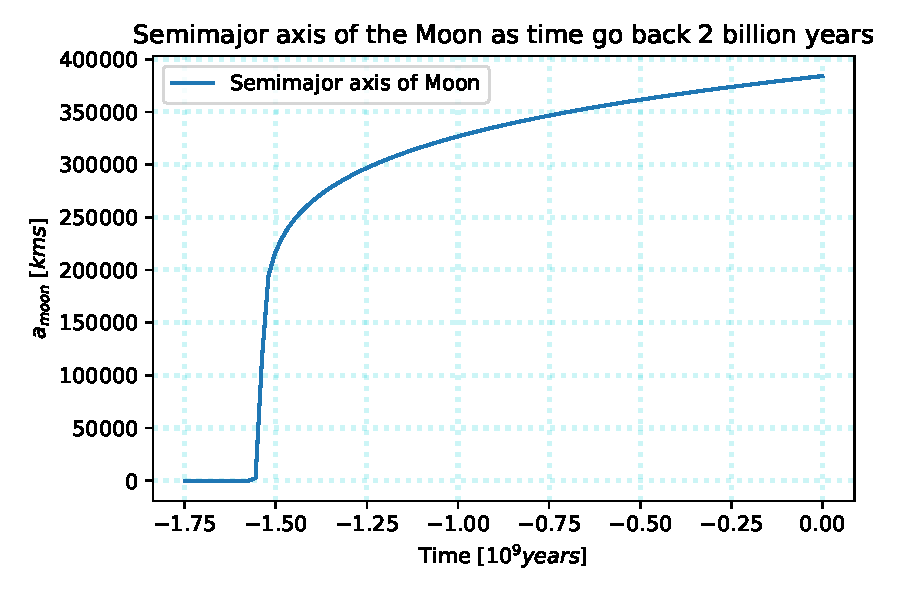
\includegraphics[scale=0.80]{plot1.pdf}
\caption{Plot of Semimajor axis vs. Time for time going back 2 billion years into the past}
\end{figure}

\begin{figure}[H]
\centering
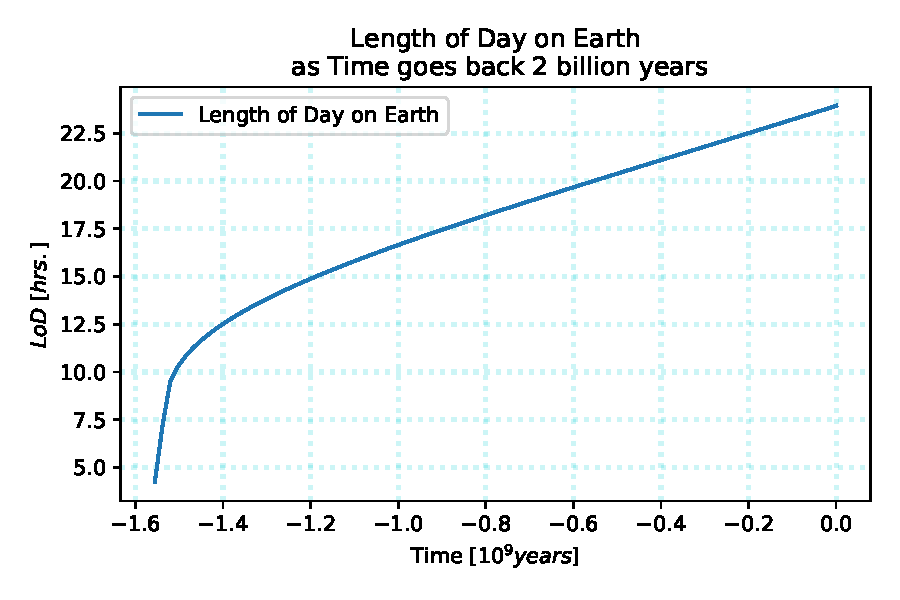
\includegraphics[scale=0.80]{plot2.pdf}
\caption{Plot of the Length of Day on Earth vs.Time for time going back 2 billion years into the past}
\end{figure}

 It is believed that the Moon formed just outside the Roche radius. Assuming this is true, the length of day on Earth at the time of the Moon's formation was found to be $8.5$ hours long.
 
 Using estimates from NASA's website, the age of the Earth is $4.54$ billion years old and the Moon is $4.51$ billion years old. These values are much older than values obtained from the tidal model.
 
 The disagreement between the tidal model and the estimates from NASA maybe due to the tidal model not incorporating the effects of other celestial objects, like gravity from other planets. Although the effects of the other celestial objects are small due to the large scales in distance, these small effects compound when integrating over billions of years. For this model the dimensionless tidal quality factor $Q_{\leftmoon}$ was assumed to be constant through time, however, one would expect this quantity to increase as the Earth and Moon got closer, since the gravitational attraction would increase as the distance between the Earth and Moon decreased. Also, changes in eccentricities were not taken into account in the system, for example, when the Earth and Moon are closer together the orbital eccentricity of their orbits would be exaggerated due to greater gravitation attraction between them this can greatly effect the angular momentum and spin angular momentum. Assuming the great impact hypothesis is true, right after the collision there was Earth and a disk of debris orbit Earth as a result of the collision. The Tidal model does not consider how this disk of debris may have formed into the Moon. This model assumes the Earth and Moon being tidally locked from the moment of impact. This assumption would not be correct when utilizing the great impact hypothesis. The process of becoming tidally locked would have rearranged the angular momentum in the Earth-Moon system. 
 
 Additionally, this model only takes into account the angular momentum of the Earth and Moon and spin angular momentum of the Earth. The energy of the system is considered. For example, energy being converted to heat in oceans due to friction can accumulate to loss of angular momentum over billions of years. 
\end{document}
